\documentclass{beamer}
\usetheme{Warsaw}

\usepackage[utf8]{inputenc}
\usepackage{fancybox}
\usepackage{multimedia} 
\usepackage{subfig}
\usepackage{amsmath}
\usepackage{hyperref}
\hypersetup{
    colorlinks=true,     
    urlcolor=blue
}
\usepackage[all]{xy}

\setbeamertemplate{footline}[frame number]


\begin{document}


\title[Stochastik] % (optional, only for long titles)
{Wahrscheinlichkeitstheorie und Statistik (Stochastik)
\\
\includegraphics[scale=0.5]{img/craps}
}
\subtitle{}
\author[Dr. Johannes Riesterer] % (optional, for multiple authors)
{Dr.  rer. nat. Johannes Riesterer}

\date[KPT 2004] % (optional)
{}

\subject{Stochastik}

\frame{\titlepage}


\begin{frame}
    \frametitle{Einleitung}
\framesubtitle{}

\begin{block}{Motivation}
Maschinelles Lernen. Maschinelle Vorhersage. Informationstheorie. Prozesstheorie. Optimierungstheorie. Mustererkennung. Komplexitätstheorie, bildgebende Verfahren, Physik.
\end{block}

\begin{block}{Motivation}

Wie programmiere und trainiere ich einen "intelligenten" Spam-Filter?
Ab wie vielen richtig beantworteten Ja-Nein-Fragen ist der  von meinem Kommilitonen gebaute Roboter wirklich intelligent und  hat nicht nur zufällig die richige Antwort gewählt?
Wie bewertet Google Webseiten?
Warum wird das Rauschen von Sensoren ständig als Normalverteilt angenommen?
Macht es Sinn auf Rot zu setzen, nachdem 100 mal Schwarz im Roulette fiel?
Kann man Geschwafel quantifizieren?
Wie kann man mit einer Münze Integrale lösen und was hat das mit Hollywood zu tun? 
\end{block}

 \end{frame}


\begin{frame}
    \frametitle{Einleitung}
\framesubtitle{Was ist Stochastik?}
    \begin{block}{Wahrscheinlichkeitstheorie}
 Beschreibung und Untersuchung von zufälligen Vorgängen und Modellen.
\end{block}
    \begin{block}{Statistik}
Umgang mit dem Zufall und Schlussfolgern aus Beobachtungen
\end{block}
 \end{frame}

\begin{frame}
    \frametitle{Einleitung}
\framesubtitle{}
    \begin{block}{Mathematik und Realität}

\begin{figure}[htp]
      \centering
    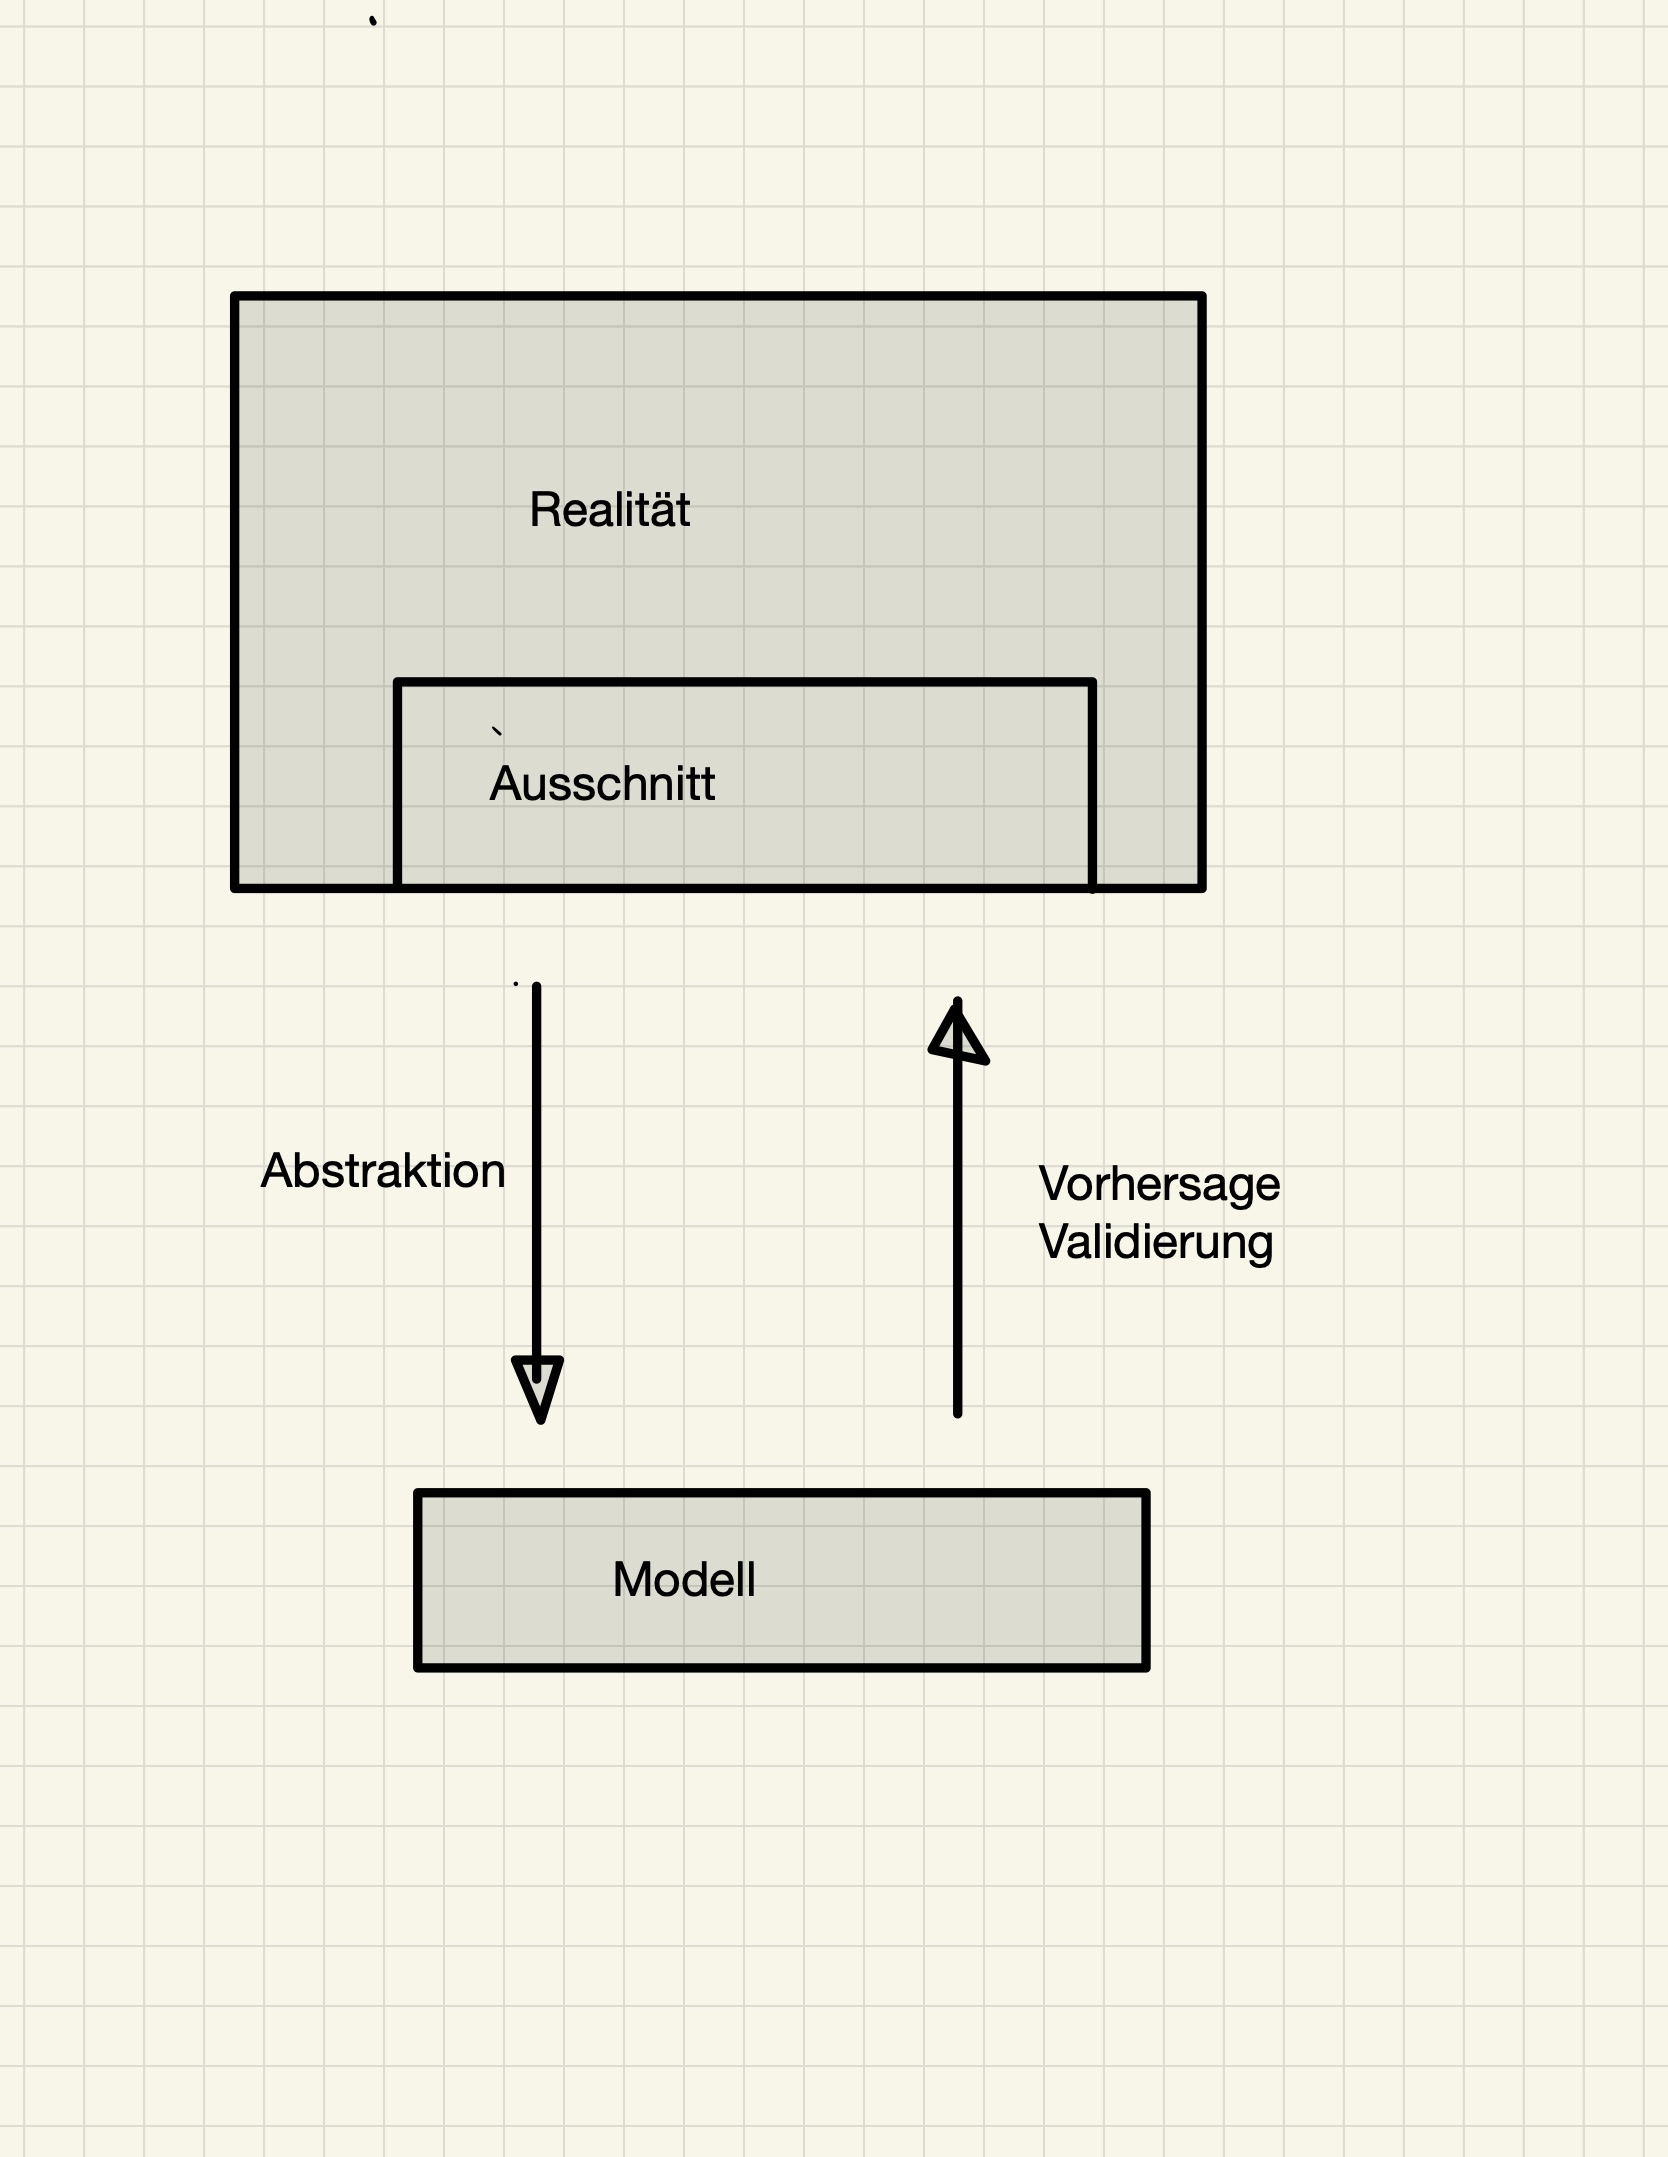
\includegraphics[width=0.5 \textwidth]{img/modellierung}

 
\end{figure}
\end{block}
 
 \end{frame}


\begin{frame}
    \frametitle{Einleitung}
\framesubtitle{}

    \begin{block}{Was ist Zufall}
Keine kausale Erklärung für den Ausgang eines Vorganges vorhanden (Nicht-Deterministisch)
\end{block}



   \begin{block}{Kausalität (Wikipedia)}
Kausalität ist die Beziehung zwischen Ursache und Wirkung. Sie betrifft die Abfolge von Ereignissen und Zuständen, die aufeinander bezogen sind. Demnach ist A die Ursache für die Wirkung B, wenn B von A herbeigeführt wird.
Eine Ursache ist zeitlich immer vor der Wirkung.
\end{block}

\begin{figure}[htp]
      \centering
    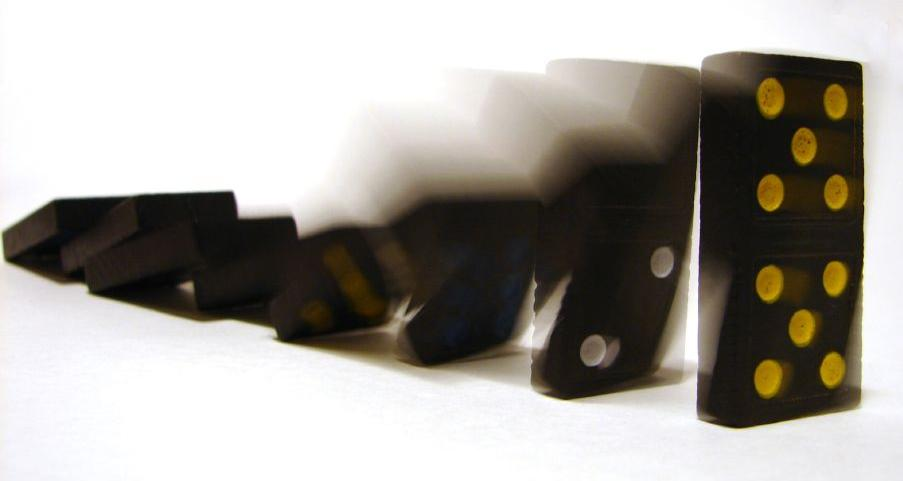
\includegraphics[width=0.3\textwidth]{img/Domino}

      \caption{Quelle: Wikipedia}
\end{figure}


\end{frame}


\begin{frame}
    \frametitle{Einleitung}
\framesubtitle{}

\begin{block}{Korrelation}
Die Korrelation beschreibt den statistischen Zusammenhang zwischen zwei Variablen – also, wie stark und in welcher Richtung sie gemeinsam variieren
\end{block}

\begin{block}{ Kausalität -> Korrelation}
Gibt es einen kausalen Zusammenhang zwischen zwei Variablen, so ist auch eine Korrelation gegeben. 
\end{block}
   
\begin{block}{Korrelation ? Kausalität}
    In den seltensten Fällen lassen sich aus Korrelationen  direkt kausale Zusammenhänge ableiten. 
    Hierfür sind weitere detallierte Schritte nötig (später mehr).
    ACHTUNG: Populisten tun dies jedoch ständig!
    \end{block}

\end{frame}






\begin{frame}
    \frametitle{Einleitung}
\framesubtitle{}

    \begin{block}{Korellation vs. Kausalität}
Beobachtung: Bei Regen tragen die Menschen einen Regenschirm.
Es folgt NICHT: Wenn man einen Regenschirm aufspannt, fängt es an zu regnen.
Ebenso folgt NICHT: Wenn es regnet, sieht man Menschen mit Regenschirmen. 
\end{block}


\begin{figure}[htp]
      \centering
    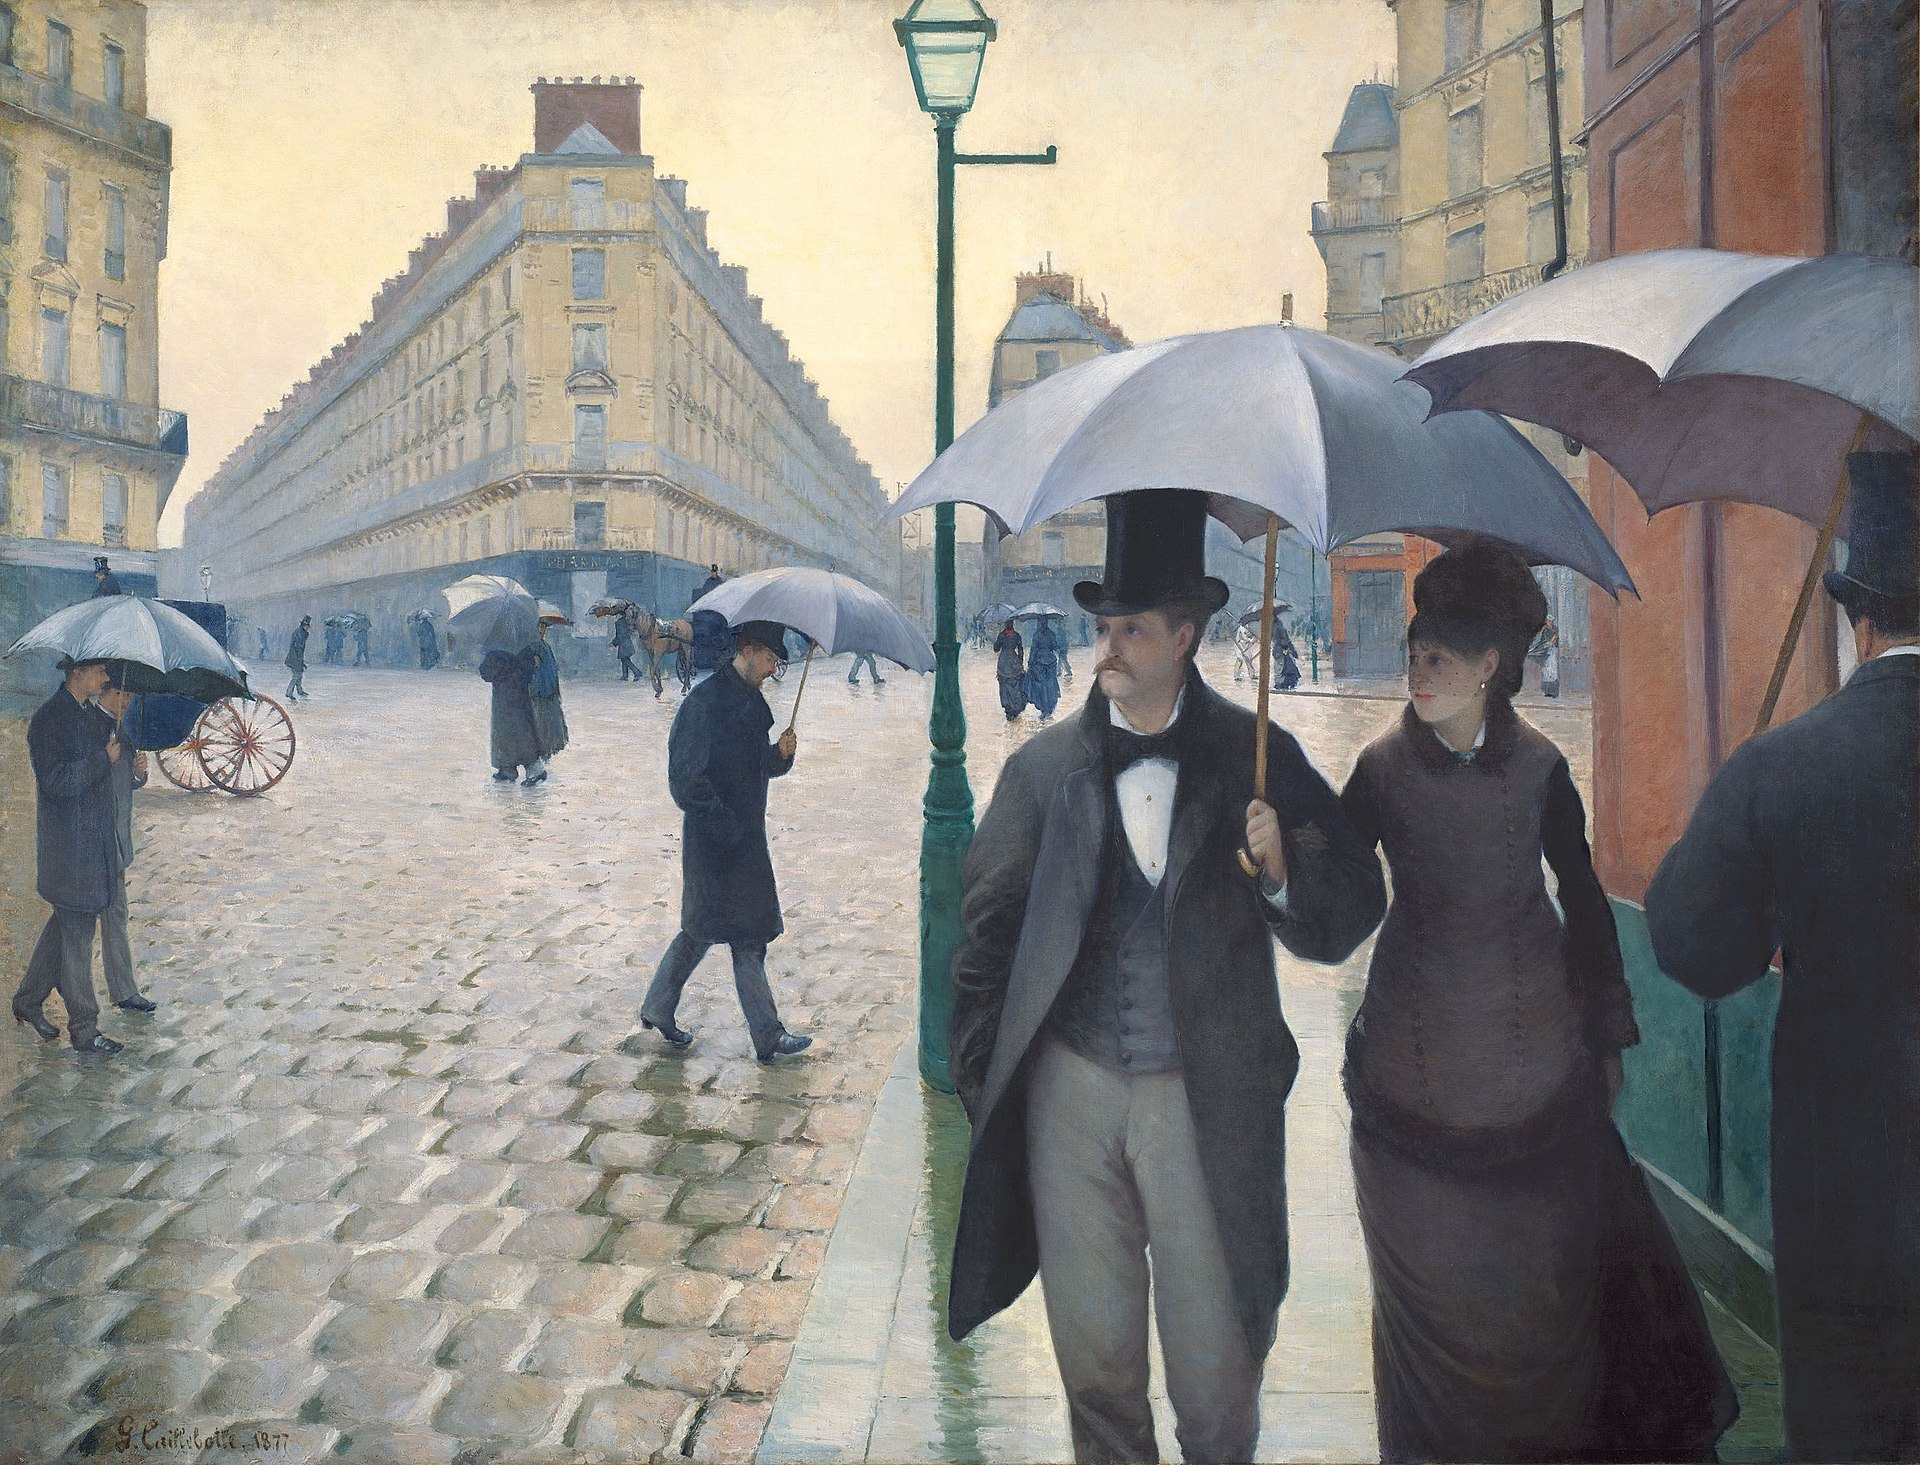
\includegraphics[width=0.6\textwidth]{img/Paris}

      \caption{Quelle: Wikipedia}
\end{figure}


\end{frame}


\begin{frame}
    \frametitle{Einleitung}
\framesubtitle{}

    \begin{block}{kreuzkorrelation}
Zwei Ereignisse treten zusammen auf, haben jedoch andere gemeinsame Ursachen.
\end{block}

%\begin{block}{Korellation vs. Kausalität}
%Um aus einer Korrelation einen kausalen Zusammenhang  ableiten zu können,  muss man alle anderen möglichen Ursachen ausschliessen.    
%\end{block} 

\begin{figure}[htp]
      \centering
    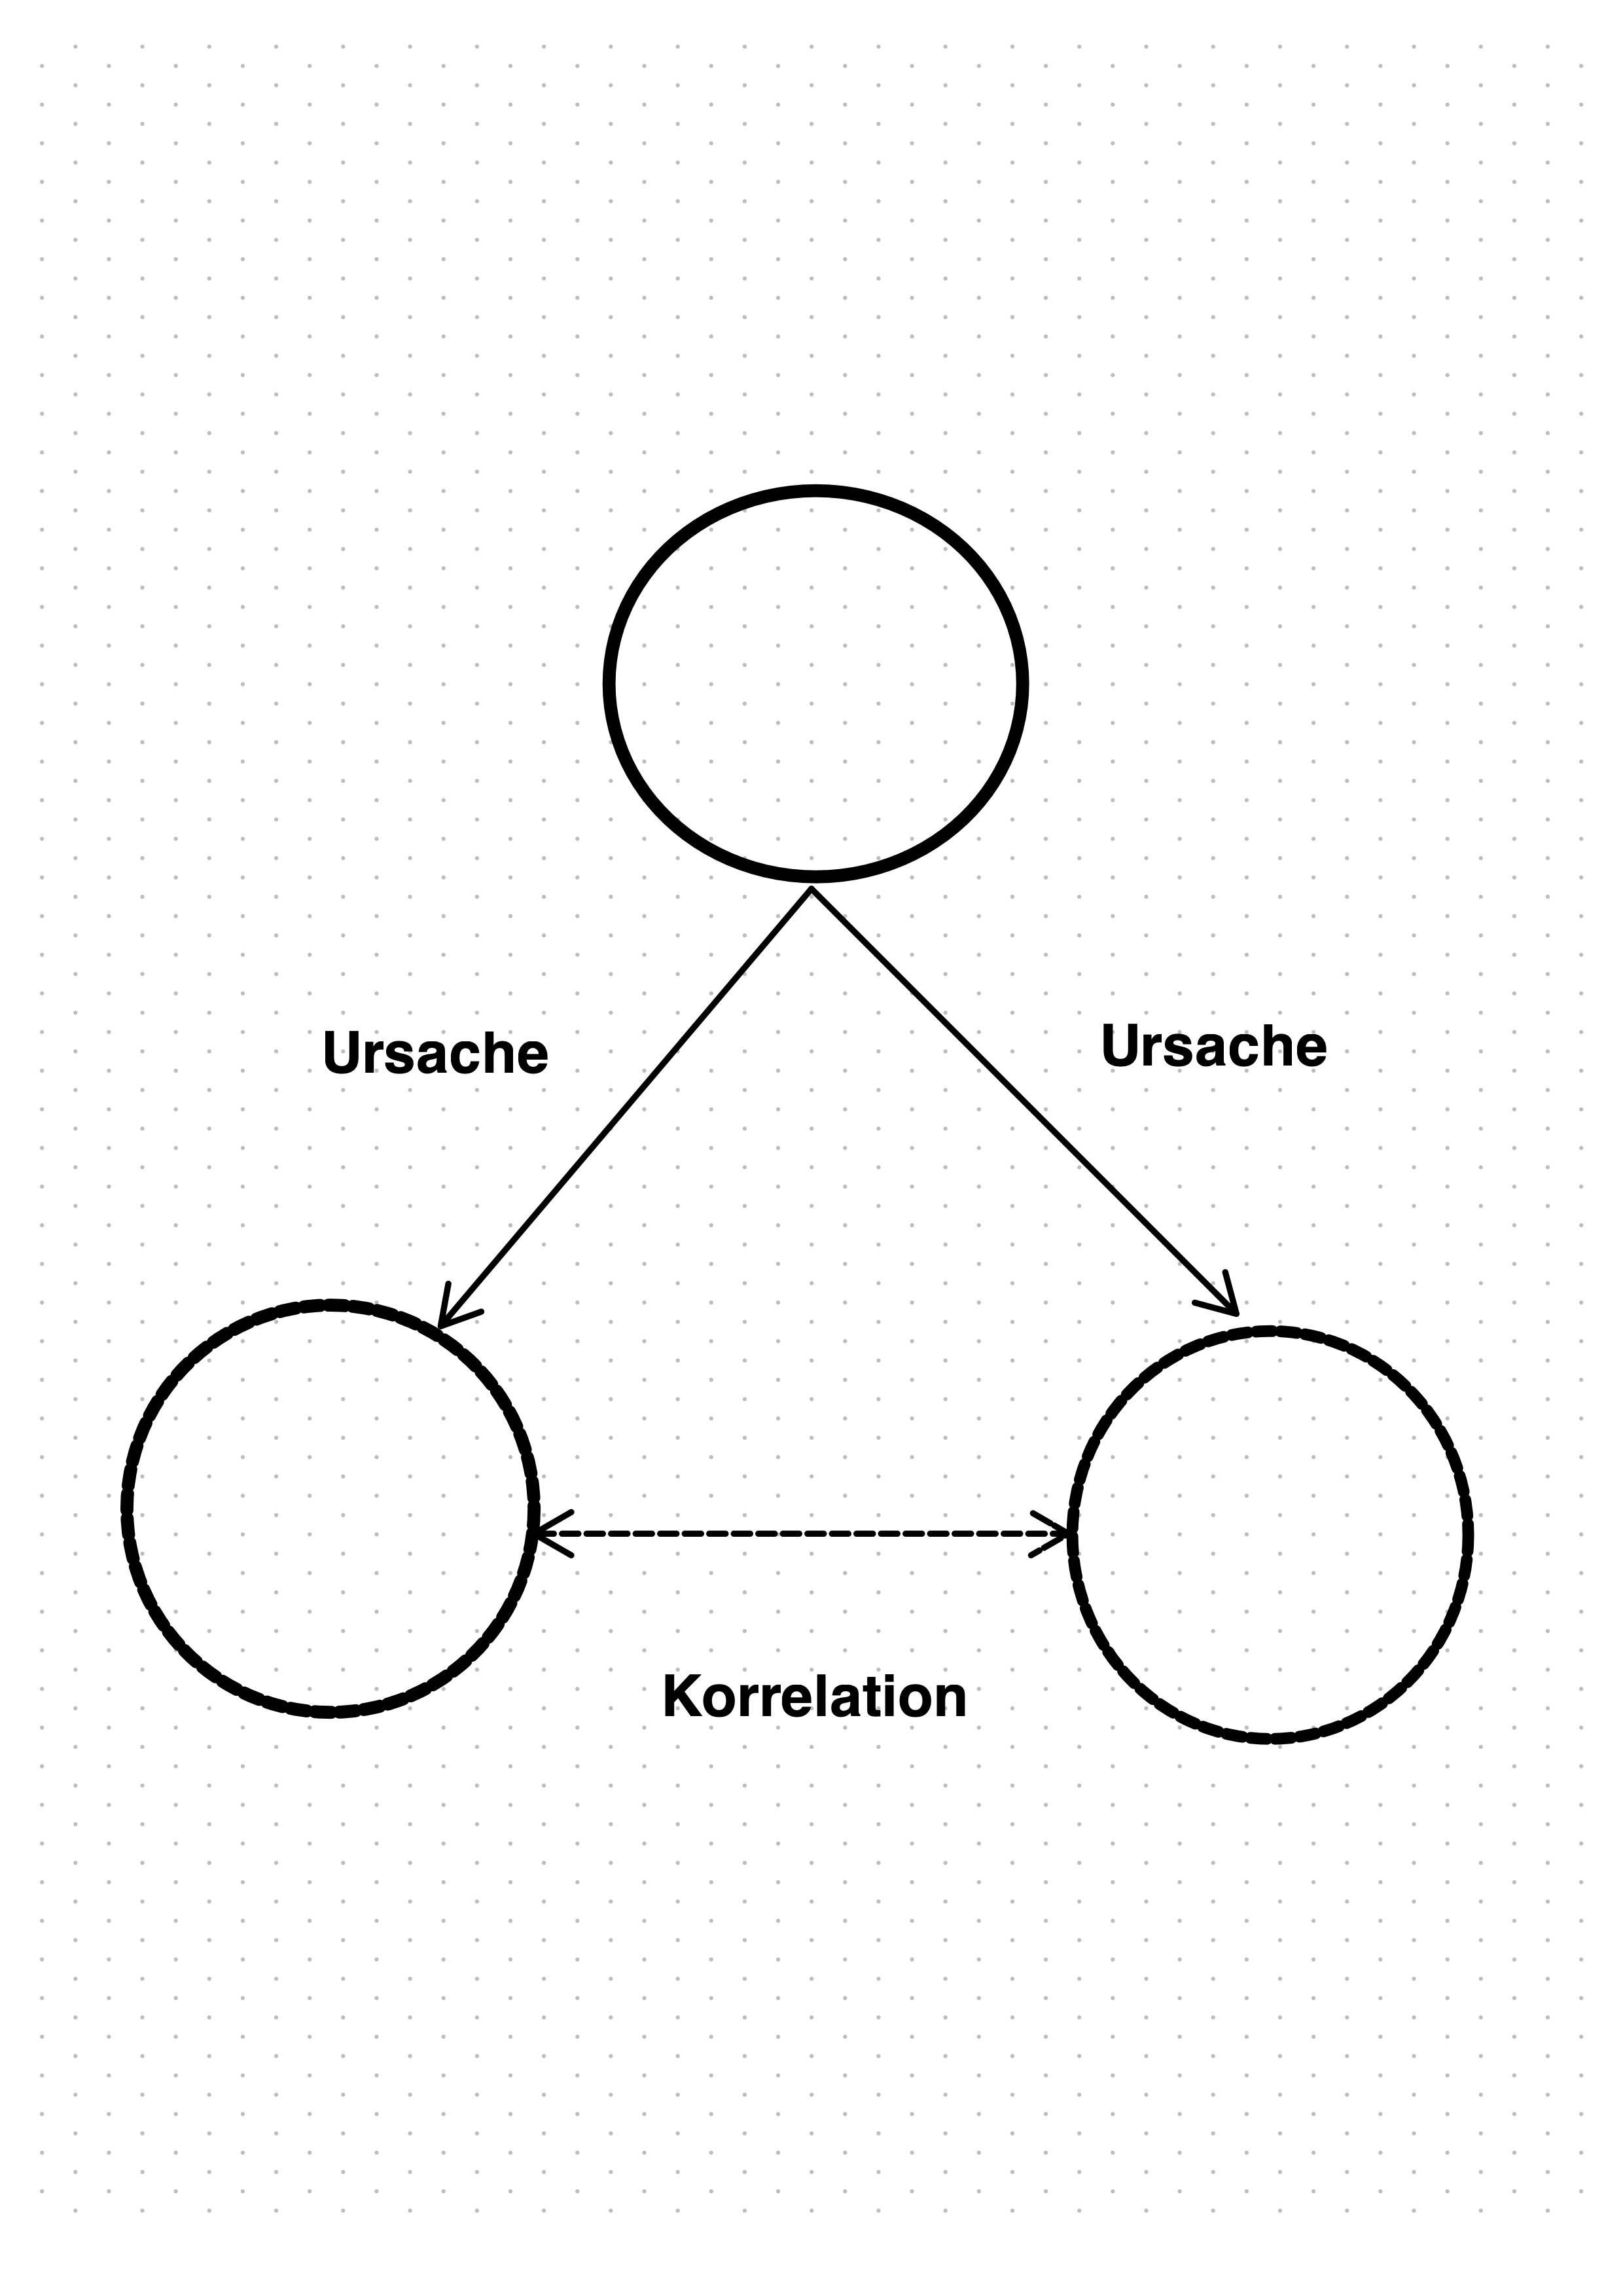
\includegraphics[width=0.33\textwidth]{img/kreuzkorrelation-2.png}

\end{figure}
\end{frame}



\begin{frame}
    \frametitle{Einleitung}
\framesubtitle{}

\begin{block}{Beispiel}
    Behauptung (falsch): Größere Füße führen zu besserem Leseverständnis.

Korrelation: Bei kleinen Kindern mit wachsendem Alter steigen sowohl Schuhgröße als auch Lesekompetenz.

Tatsächlicher Grund: Alter ist die dritte Variable – ältere Kinder können besser lesen und haben größere Füße.

\end{block}


\end{frame}


\begin{frame}
    \frametitle{Einleitung}
\framesubtitle{}

\begin{block}{Kontrolliertes Experiment}
    Ein kontrolliertes Experiment ist eine Untersuchungsmethode, 
    bei der eine Variable (die unabhängige Variable) gezielt manipuliert wird, 
    um deren Einfluss auf eine andere Variable (die abhängige Variable) zu beobachten. 
    Dabei werden alle anderen Einflussgrößen konstant gehalten oder   Randomisiert.
    Dies ermöglicht eine klare Zuordnung von Ursache und Wirkung.    
\end{block}


\end{frame}



\begin{frame}
    \frametitle{Einleitung}
\framesubtitle{}
\begin{block}{}
Gibt es überhaupt Zufall oder steht alles in einem kausalen Zusammenhang? 
\end{block}

\begin{figure}[htp]
      \centering
    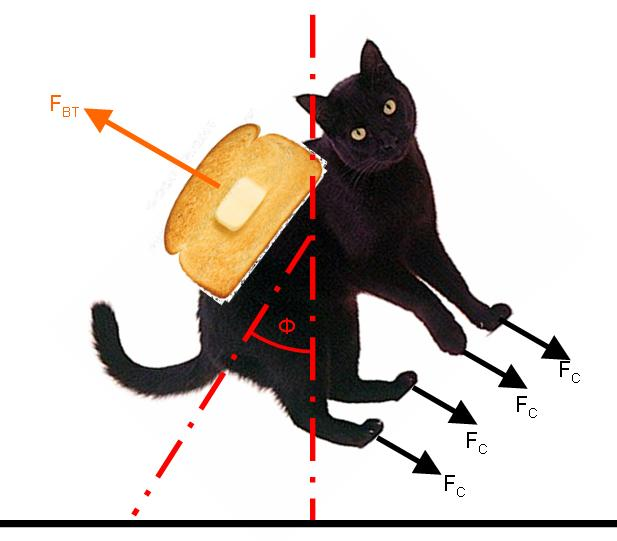
\includegraphics[width=0.2\textwidth]{img/katze-toast}

      \caption{Quelle: https://www.laurentinews.de/wp-content/uploads/2014/03/katze-toast1.jpg}
\end{figure}

    \begin{block}{}
Zufall hängt von der betrachteten Skala ab. \\
Physik $\Rightarrow$ Skalen können nicht beliebig klein werden.
\end{block}
    \begin{block}{}
\href{https://de.wikipedia.org/wiki/Brownsche_Bewegung
}{Wikipedia://Brownsche Molekularbewegung.
}
\end{block}

\end{frame}



\begin{frame}
    \frametitle{Einleitung}
\framesubtitle{}

\begin{block}{Literatur}
\begin{itemize}
\item Stochastik für Informatiker; L. Dümbgen; Springer
\item Einführung in die Wahrscheinlichkeitstheorie und Statistik; Hans-Otto Georgii; De Gruyter Studium
\item Achim Klenke; Wahrscheinlichkeitstheorie; Springer
\end{itemize}
\end{block}


 \end{frame}



\begin{frame}
    \frametitle{Highlight}
\framesubtitle{}
\begin{figure}[htp]
      \centering
    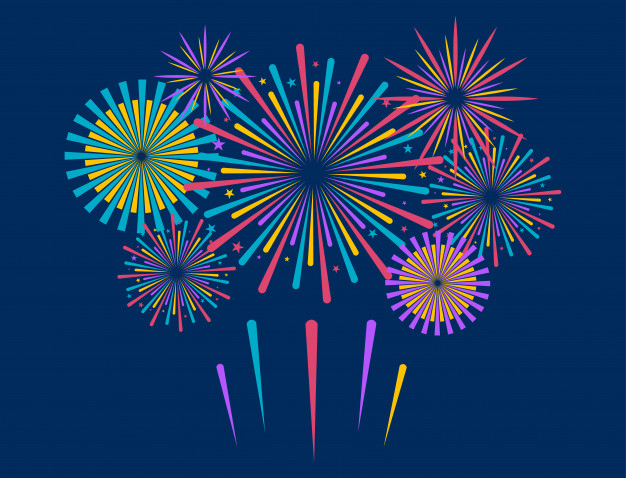
\includegraphics[width=0.9\textwidth]{img/firework}
\end{figure}
 \end{frame}


\begin{frame}
    \frametitle{Einleitung}
\framesubtitle{}

\begin{block}{Bessere Entscheidungen durch Mathematik?!?}
Gegeben sind 3 geschlossene Türen.  Hinter einer ist der Hauptgewinn, hinter zwei eine Ziege.
Der Spieler darf  sich zuerst für eine Tür entscheiden. 
Danach öffnet der Moderator eine der  nicht gewählten Türen, hinter der nicht der Hauptgewinn ist und fragt den Spieler, oben er seine vorige Entscheidung revidieren und die andere geschlossene Tür öffnen möchte.
\end{block}

\begin{figure}[htp]
      \centering
    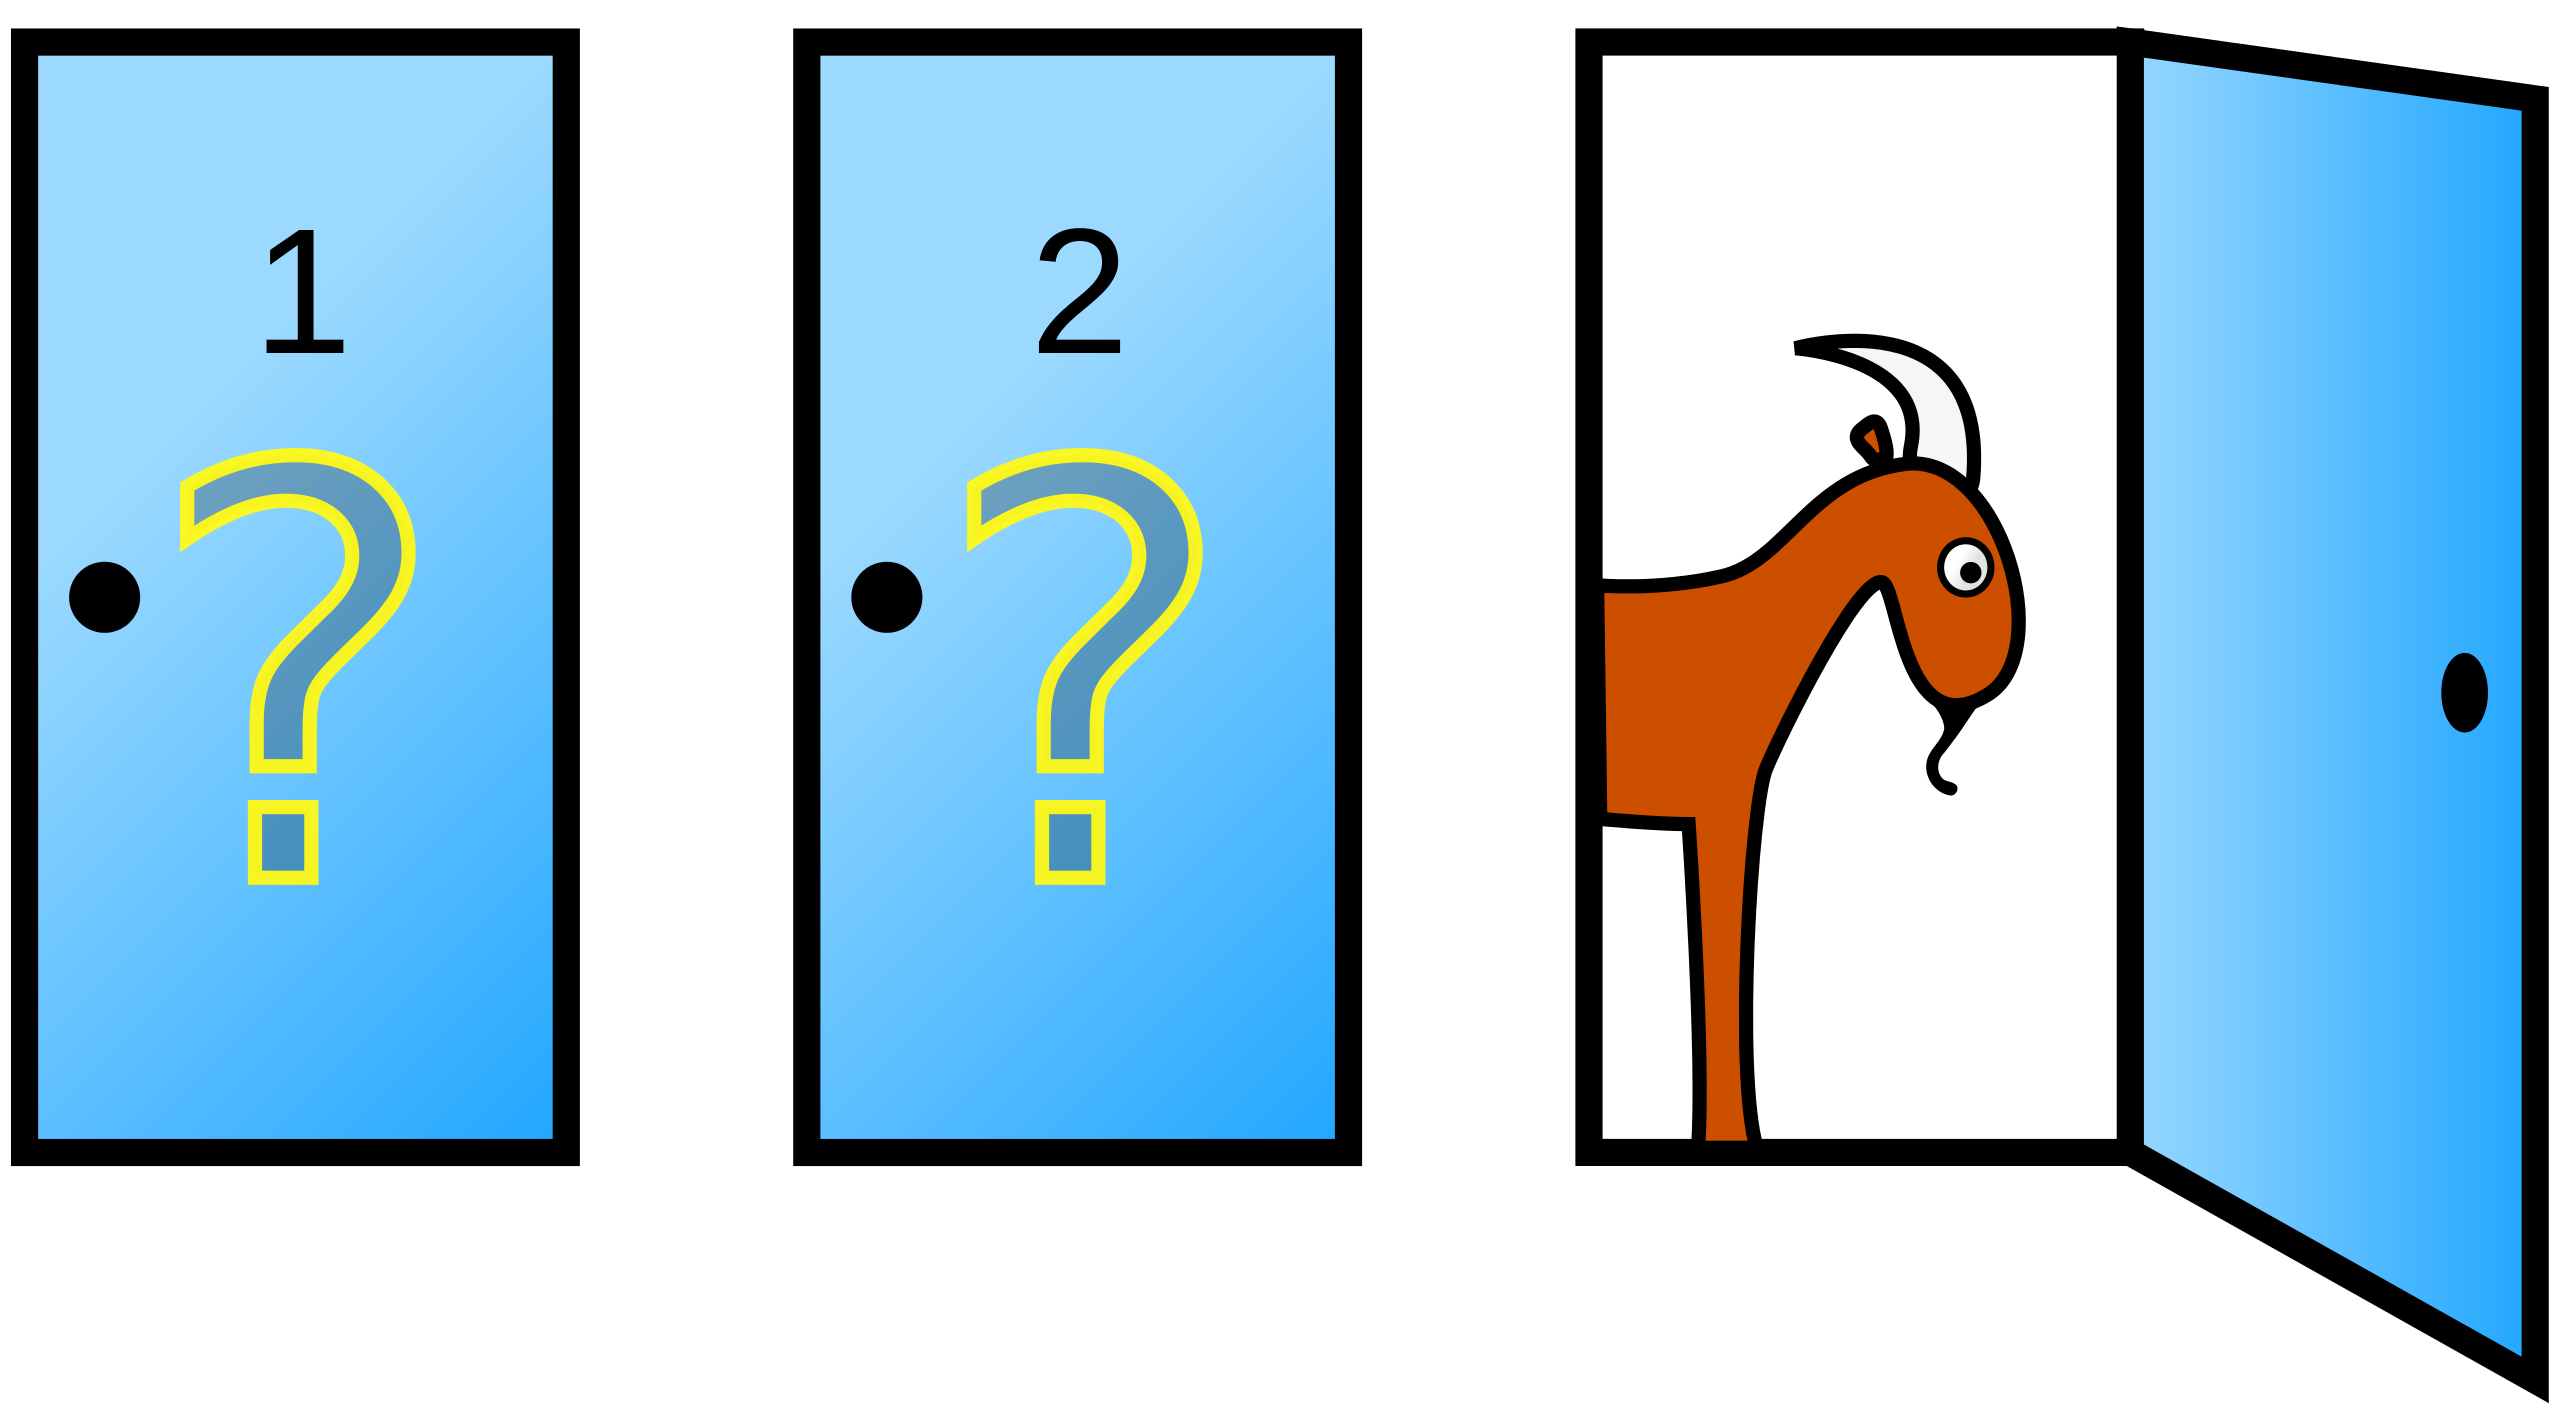
\includegraphics[width=0.45\textwidth]{img/Monty_open}

      \caption{Quelle: Wikipedia}
\end{figure}

 \end{frame}

\begin{frame}
    \frametitle{Einleitung}
\framesubtitle{}

\begin{block}{Bessere Entscheidungen durch Mathematik?!?}
Hat der Spieler eine höhere Gewinnchance, wenn er die Tür wechselt?
\end{block}

 \end{frame}

\begin{frame}
    \frametitle{Einleitung}
\framesubtitle{}

\begin{block}{Bessere Entscheidungen durch Mathematik?!?}
Wechseln hat eine höhere Gewinnchance!
\end{block}

\begin{figure}[htp]
      \centering
    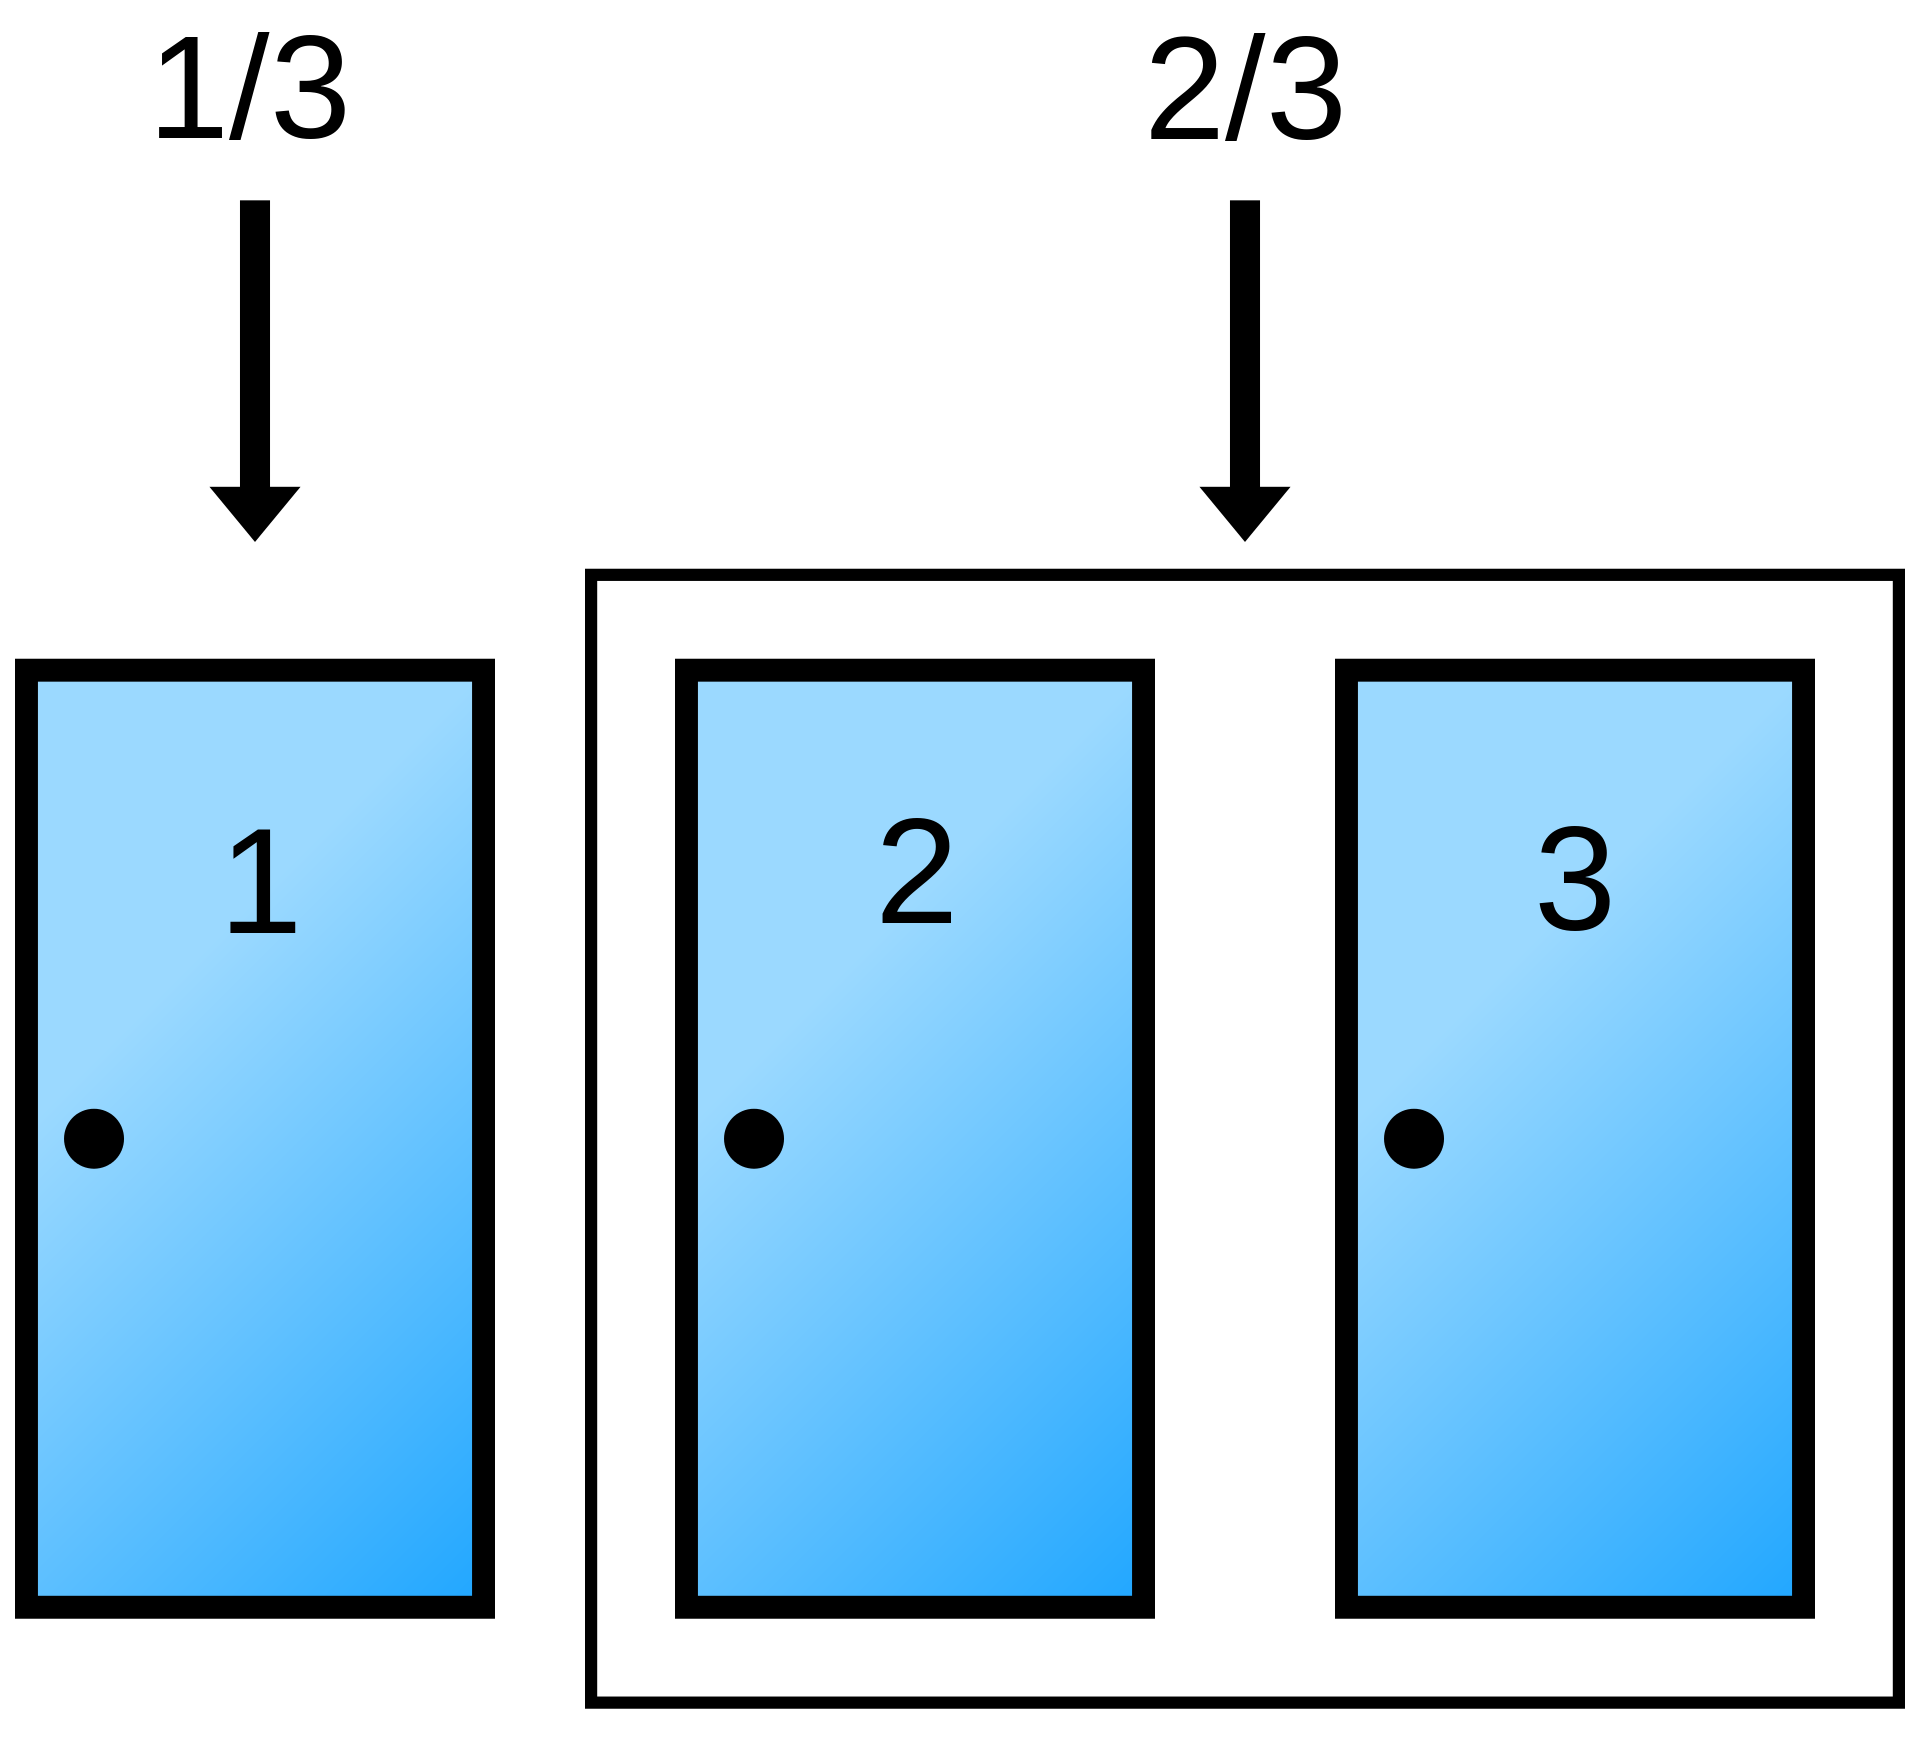
\includegraphics[width=0.45\textwidth]{img/Monty_closed_1}
    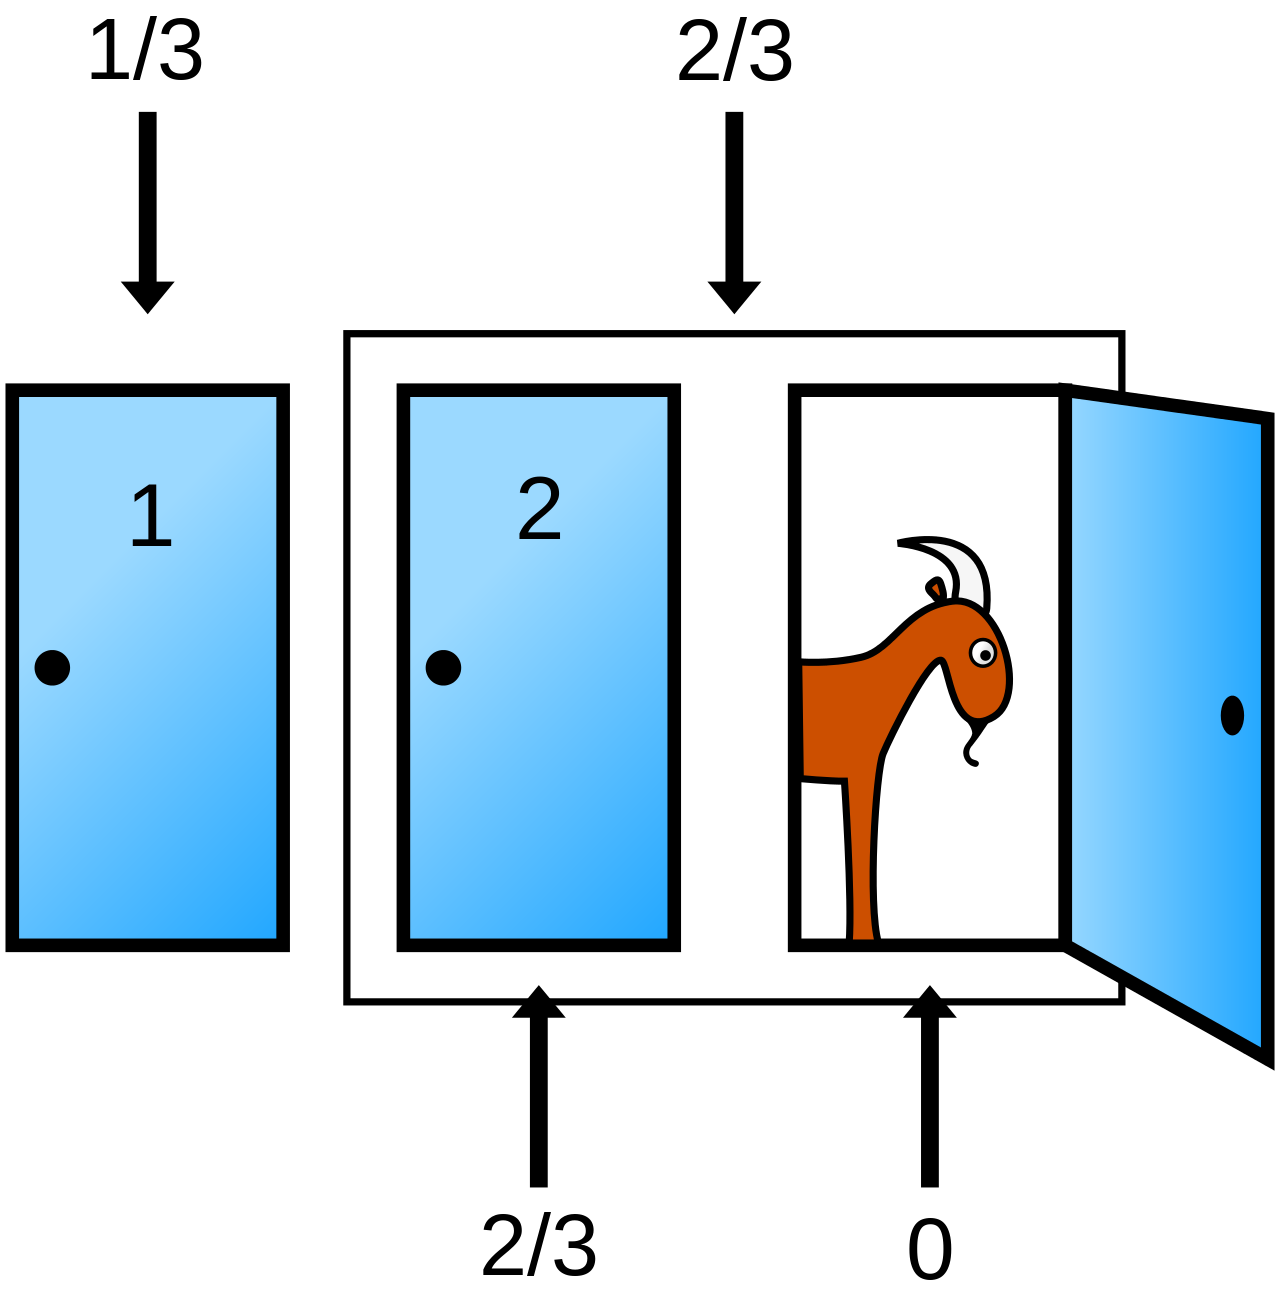
\includegraphics[width=0.45\textwidth]{img/Monty_open_1}
      \caption{Quelle: Wikipedia}
\end{figure}

 \end{frame}



 \begin{frame}
    \frametitle{Einleitung}
\framesubtitle{}


\begin{figure}[htp]
      \centering
    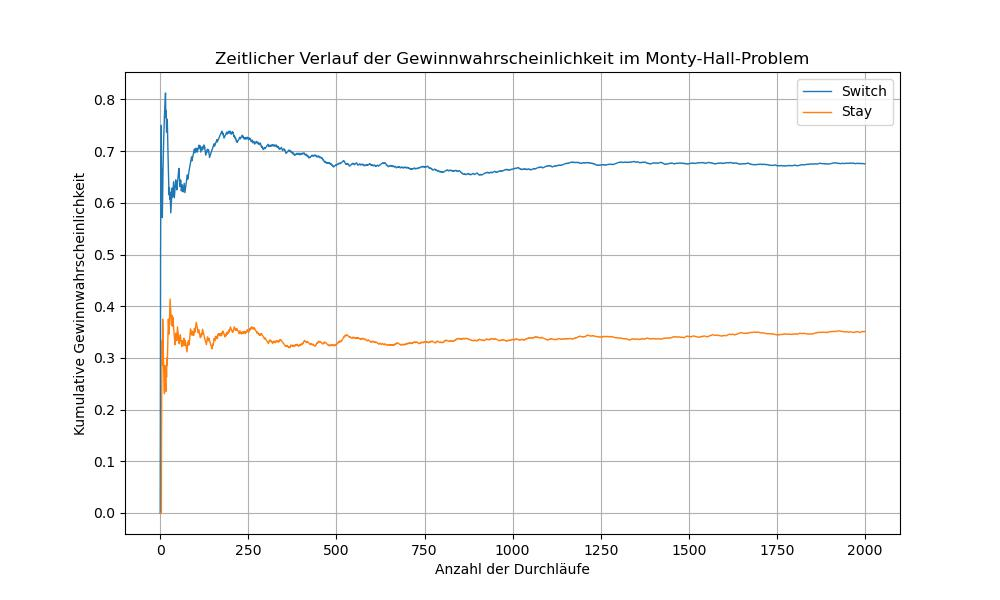
\includegraphics[width=0.95\textwidth]{img/montyhall.jpg}
\end{figure}

 \end{frame}

\end{document}
